\documentclass{article}

% Draft against the official NeurIPS style (workshops use the same layout).
% At submission time: swap neurips_2023.sty for the target workshop's file
% and drop the [preprint] option to anonymize.
\usepackage[preprint]{neurips_2023}

\usepackage[utf8]{inputenc}
\usepackage[T1]{fontenc}
\usepackage{hyperref}
\usepackage{url}
\usepackage{booktabs}
\usepackage{amsmath, amssymb}
\usepackage{xcolor}
\usepackage{graphicx}
\usepackage{tikz}
\usetikzlibrary{arrows.meta, positioning, calc}
\usepackage{microtype}
\usepackage{enumitem}

\newcommand{\todo}[1]{\textcolor{orange!75!black}{\textbf{[TODO: #1]}}}
\newcommand{\se}{\textnormal{\textsc{se}}}
\newcommand{\bon}{\textnormal{\textsc{b}o\textsc{n}}}
\newcommand{\pass}[1]{pass@#1}

\title{Beyond the Sampling Frontier: Distilling Test-Time\\ Evolutionary Discoveries into Generalizable Coding Capability}

\author{%
  Mian Wu \\
  \todo{affiliation} \\
  \texttt{tuboushuu@gmail.com} \\
  \And
  \todo{co-authors (Harman, \ldots) and affiliations} \\
}

\begin{document}

\maketitle

\begin{abstract}
Test-time search---from repeated sampling to evolutionary refinement against execution feedback---lets language models solve programming problems far beyond single-sample reach. But search improves only the instance at hand, and its cost recurs on every new problem. We ask whether test-time discoveries can be converted into \emph{persistent} capability: does fine-tuning on solutions discovered by test-time evolution generalize to unseen problems? Under acquisition-matched conditions (same source pool, generation budget, SFT recipe, and held-out evaluation), SFT on solutions discovered by Squeeze-Evolve (\se{}), an oracle-verified evolutionary search, lifts a held-out hard-frontier set from 20 to 26--29 solved of 457 across three seeds, while SFT on Best-of-$N$ data stays at 20--21. We trace the gap to \emph{support expansion}: only $3.4\%$ of Best-of-$N$'s usable rows lie beyond ordinary sampling reach, versus $40.7\%$ for \se{}, so na\"ive self-training feeds the model what it already knows---a capability-selection bias that evolutionary search breaks. Distillation is not free: we document a mild, statistically insignificant distribution-sharpening cost on a general dev set ($189 \to 185$--$188$ of $200$) and show that a low-dose refit recovers most of it while keeping most of the frontier gain. \emph{Search gains} and \emph{learnable gains} are distinct axes; we outline family-balanced distillation for converting more of the former into the latter.
\end{abstract}

\section{Introduction}
\label{sec:intro}

Scaling test-time compute reliably extends what language models can solve. Repeated sampling alone raises coverage on reasoning and coding benchmarks \citep{chen2021codex, brown2024monkeys, snell2024scaling}, and richer procedures---self-refinement \citep{madaan2023selfrefine, shinn2023reflexion}, execution-guided repair \citep{olausson2024selfrepair}, and evolutionary search over programs \citep{romera2024funsearch, novikov2025alphaevolve}---push further still: with a reliable verifier, search reaches solutions that the base policy essentially never samples. That search with oracle verification finds more solutions is, however, largely established---and unsatisfying on its own: the gain is paid again on every instance and leaves no trace in the weights.

The natural next step is to distill search outputs back into the model \citep{zelikman2022star, yuan2023scaling, gulcehre2023rest, singh2023beyond}. But na\"ive self-training carries a subtle failure mode: \emph{the policy selects its own training data}. Under ordinary sampling, the probability that a problem contributes a verified solution is the model's own solve rate on it; problems at the capability frontier, where $p_\theta(\text{success}) \approx 0$, almost never enter the training set. Self-training therefore feeds the model more demonstrations of what it already does---a \emph{capability-selection bias} that concentrates probability mass on known modes rather than extending them (cf.\ diversity loss under preference tuning \citep{kirk2024understanding}).

This paper asks the question we believe matters most for test-time search: \textbf{can solutions discovered by test-time evolution---specifically $0{\to}1$ discoveries that ordinary sampling fails to reach---be distilled into capability that transfers to unseen problems?} We deliberately separate two axes that are often conflated:
\emph{search gain}, solving more instances at inference time, and \emph{learnable gain}, the downstream training value of the trajectories found. A method can deliver the former without the latter.

\paragraph{Contributions.}
\begin{enumerate}[leftmargin=*, itemsep=1pt, topsep=2pt]
  \item \textbf{An acquisition-matched comparison.} With the source problem pool, generation budget, verification, SFT recipe, and evaluation all held fixed, SFT on \se{}-discovered solutions raises a held-out frontier set from $20$ to $26$--$29$ solved of $457$ (three seeds), while Best-of-$N$ SFT stays at $20$--$21$---non-overlapping seed distributions (\S\ref{sec:main}).
  \item \textbf{A provenance analysis.} The gain traces to data beyond ordinary sampling reach: $40.7\%$ of \se{}'s frontier-slice rows are solutions no ordinary-sampling pipeline found, versus $3.4\%$ in easier slices; per-problem decomposition shows the improvement comes from newly solved problems, not uniform lift (\S\ref{sec:provenance}).
  \item \textbf{Honest cost accounting.} Distillation mildly \emph{sharpens} the output distribution: on a $200$-problem general dev set, correct samples can rise while covered problems fall ($189 \to 185$--$188$; insignificant, concentrated in the hardest slice). The effect is dose-dependent, and a low-dose refit restores dev coverage while keeping most of the frontier gain (\S\ref{sec:cost}).
  \item \textbf{A distillation roadmap.} We analyze why the current recipe sharpens (single-reference targets, unsupervised thinking, unmatched thinking budgets) and propose family-balanced, insight-first, per-problem-normalized multi-solution distillation (\S\ref{sec:roadmap}).
\end{enumerate}

\begin{figure}[t]
\centering
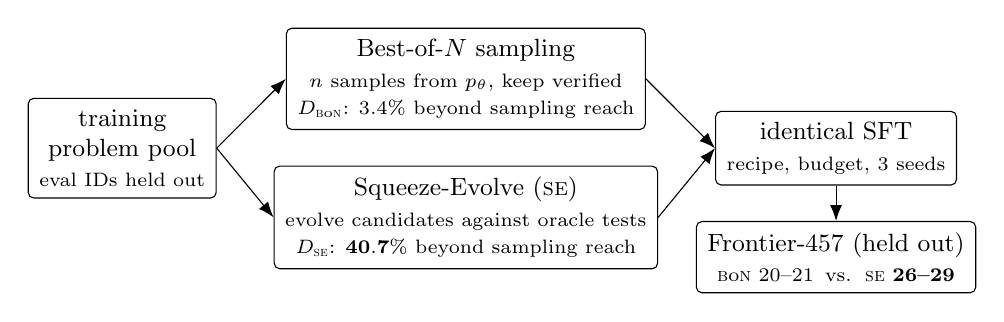
\begin{tikzpicture}[
  font=\small,
  box/.style={draw, rounded corners=2pt, align=center, inner sep=4pt},
  >={Latex[length=2mm]}
]
  \node[box] (bon) {Best-of-$N$ sampling\\ \scriptsize $n$ samples from $p_\theta$, keep verified\\[-1pt] \scriptsize $D_{\bon{}}$: $3.4\%$ beyond sampling reach};
  \node[box, below=4.5mm of bon] (se) {Squeeze-Evolve (\se{})\\ \scriptsize evolve candidates against oracle tests\\[-1pt] \scriptsize $D_{\se{}}$: $\mathbf{40.7\%}$ beyond sampling reach};
  \node[box, left=8mm of {$(bon.west)!0.5!(se.west)$}, anchor=east] (pool) {training\\ problem pool\\ \scriptsize eval IDs held out};
  \node[box, right=8mm of {$(bon.east)!0.5!(se.east)$}, anchor=west] (sft) {identical SFT\\ \scriptsize recipe, budget, $3$ seeds};
  \node[box, below=4.5mm of sft] (eval) {Frontier-457 (held out)\\ \scriptsize \bon{} 20--21 \,vs.\, \se{} \textbf{26--29}};
  \draw[->] (pool.east) -- (bon.west);
  \draw[->] (pool.east) -- (se.west);
  \draw[->] (bon.east) -- (sft.west);
  \draw[->] (se.east) -- (sft.west);
  \draw[->] (sft) -- (eval);
\end{tikzpicture}
\caption{\textbf{Acquisition-matched design.} Everything is matched except \emph{how} verified solutions are discovered; the resulting datasets differing is the treatment, not a confound. \se{} imports frontier problems into the training support that ordinary sampling cannot supply.}
\label{fig:pipeline}
\end{figure}

\section{From discovery to capability}
\label{sec:method}

\paragraph{Setup.}
Let $p_\theta$ be the base policy over solutions $y$ to programming problems $x$, each equipped with executable unit tests (the oracle). A solution is \emph{verified} if it passes the full test suite. We stratify problems by the base model's observed solve count over $16$ initial samples: \emph{bucket-$b$} contains problems solved $b/16$ times. Bucket-$0$ is the observable frontier; note the observation is noisy---a problem with true per-sample success rate $5\%$ still lands in bucket-$0$ with probability $(1-0.05)^{16} \approx 44\%$---so bucket-$0$ mixes genuinely hard problems, systematic blind spots, and unlucky low-probability problems.

\paragraph{Two acquisition procedures, one budget.}
\emph{Best-of-$N$ (\bon{})} draws $n$ candidates per problem from $p_\theta$, keeps verified ones, and selects one per problem. \emph{Squeeze-Evolve (\se{})} runs an iterative evolutionary loop: a population of candidate programs is executed against the oracle tests, and failing candidates are mutated, recombined, and repaired conditioned on execution feedback; verified survivors are collected. \todo{fill exact \se{} loop hyperparameters: population size, loop count, mutation operators, per-problem budget}. Solutions found for problems where every direct sample fails are \emph{$0{\to}1$ discoveries}. Both procedures see the same problem pool and comparable generation budget.

We emphasize what ``matched'' means: we match the \emph{acquisition conditions}---pool, budget, verification, formatting, SFT recipe, evaluation---but not the resulting datasets. $D_{\se{}} \neq D_{\bon{}}$ is precisely the treatment under study (Figure~\ref{fig:pipeline}); forcing the datasets to agree would delete the phenomenon, because \se{}'s effect, if any, is to change the \emph{support} of the training data.

\paragraph{Distillation.}
Unless noted, all SFT arms use the same K1 (single reference per problem) native-format recipe: the teacher-forced native reasoning trace appears in context but is loss-masked, and the loss is computed on the final solution only; $2$ epochs. These choices matter for the failure analysis in \S\ref{sec:cost}.

\section{Experimental setup}
\label{sec:setup}

\textbf{Model and data.} The student is a \todo{model name}~4B code model. The training pool contains \todo{pool size} problems with unit tests; all evaluation IDs are strictly disjoint from training (anything else would be leakage). The \se{} SFT set contains $794$ rows from the frontier (bucket-$0$) slice and $745$ rows from buckets $1$--$3$; \bon{} sets are constructed from the same pool at the same budget. \todo{data-statistics matching table: rows, unique problems, total tokens, solution length distributions for $D_{\se}$ vs.\ $D_{\bon}$.}

\textbf{Evaluations.} (a)~\emph{Frontier-457}: $457$ held-out problems on which the base model solved $0/16$ in an initial screen. (b)~\emph{Dev-200}: $200$ held-out general problems spanning four difficulty slices (1--3 hardest through 12--15 easiest), used to measure retention. Each model draws $16$ samples per problem; we report \pass{1}/\pass{8}/\pass{16} and \emph{solved} (problems with $\geq 1$ verified sample). SFT arms are trained with $3$ seeds.

\textbf{Thinking budget.} SFT models are evaluated with a forced reasoning floor of $7{,}300$ tokens. Because SFT shortens spontaneous reasoning, the compute-closest base control is the base model at floor $=0$: mean thinking on Frontier-457 is $6{,}887$ (base) vs.\ $6{,}210$--$6{,}442$ (\se{} arms).

\section{Results}
\label{sec:results}

\subsection{Main result: evolution-discovered data has training value; \bon{} data does not}
\label{sec:main}

\begin{table}[t]
\caption{\textbf{Frontier-457 (held out).} SFT on \se{}-discovered solutions moves the frontier; SFT on \bon{} data from the same pool, budget, and recipe does not. Solved ranges are over $3$ seeds; per-\pass{k} metrics from one representative seed. \todo{replace with seed means $\pm$ std; add paired bootstrap / McNemar CIs.}}
\label{tab:main}
\centering
\small
\begin{tabular}{lccccc}
\toprule
Model & Mean thinking & \pass{1} & \pass{8} & \pass{16} & Solved / 457 \\
\midrule
Base (floor $0$) & 6{,}887 & 0.520\% & 2.751\% & 4.376\% & 20 \\
\bon{}-SFT (floor $0$) & 5{,}939 & 0.424\% & 2.743\% & 4.376\% & 20 \; [20--21] \\
\se{}-SFT, standard & 6{,}210 & 0.615\% & 3.471\% & 5.689\% & 26 \; [\textbf{26--29}] \\
\se{}-SFT, tuned (hp778) & 6{,}416 & \textbf{0.848\%} & \textbf{4.018\%} & \textbf{6.346\%} & \textbf{29} \\
\se{}-SFT, low-dose refit & 6{,}442 & 0.766\% & 3.699\% & 5.470\% & 25 \\
\midrule
\multicolumn{6}{l}{\scriptsize Controls: \bon{}-SFT at floor $7{,}300$ drops to $14/457$; an over-trained \se{} arm ($15.6$ epochs, UM390) drops to $18/457$ (\S\ref{sec:cost}).} \\
\bottomrule
\end{tabular}
\end{table}

Table~\ref{tab:main} shows the central finding. Across three seeds, \se{}-SFT solves $26$--$29$ of $457$ held-out frontier problems against the base model's $20$---a $+30$--$45\%$ relative increase---with consistent lifts in \pass{1}, \pass{8}, and \pass{16}. \bon{}-SFT, trained on the same pool with the same recipe and budget, stays at $20$--$21$. The seed distributions do not overlap: $\min(\se{}) = 26 > \max(\bon{}) = 21$.

First, the improvement is not explained by ``SFT on verified code helps'': \bon{}-SFT is the direct counterexample. Collecting more correct solutions of \emph{ordinary reach} does not move the frontier. Second, because Frontier-457 is disjoint from training, the \se{} gain is generalization, not memorization: solutions discovered by evolution on \emph{other} problems teach something that transfers.

\subsection{Where the gain comes from: support expansion}
\label{sec:provenance}

\begin{table}[t]
\begin{minipage}[t]{0.52\linewidth}
\caption{\textbf{Provenance of training signal.} Share of SFT rows whose solution no ordinary-sampling pipeline found (\emph{only-\se{}}).}
\label{tab:onlyse}
\centering
\small
\begin{tabular}{lccc}
\toprule
Slice & Rows & Only-\se{} & Share \\
\midrule
bucket-$0$ & 794 & 323 & \textbf{40.7\%} \\
buckets 1--3 & 745 & 25 & 3.4\% \\
\bottomrule
\end{tabular}
\end{minipage}\hfill
\begin{minipage}[t]{0.44\linewidth}
\caption{\textbf{Per-problem decomposition} on Frontier-457 vs.\ base.}
\label{tab:decomp}
\centering
\small
\begin{tabular}{lccc}
\toprule
Arm & New & Lost & Net \\
\midrule
\se{} standard & 14 & 8 & $+6$ \\
\se{} tuned & 15 & 6 & $+9$ \\
\se{} refit & 11 & 6 & $+5$ \\
\bottomrule
\end{tabular}
\end{minipage}
\end{table}

Why does $D_{\se{}}$ teach when $D_{\bon{}}$ does not? Table~\ref{tab:onlyse} quantifies the difference in \emph{what} each pipeline can supply. In the frontier slice, $40.7\%$ of \se{}'s rows are solutions that ordinary sampling never found at this budget---genuine capability signal beyond the base policy's reach. In buckets $1$--$3$, only $3.4\%$ of rows are; the rest are extra demonstrations of what the model already does. \bon{} data is, by construction, the second kind everywhere.

This supports a simple account. Ordinary self-training samples training data \emph{through} $p_\theta$, so its support is confined to $\{x : p_\theta(\text{success}\,|\,x) \gg 0\}$; the gradient then re-concentrates mass on already-typical modes. Evolution uses external execution feedback to raise success probability \emph{at} the frontier, expanding the training support ($D_{\text{reachable}} \to D_{\text{reachable}} \cup D_{\text{frontier}}$); SFT then moves $p_{\theta'}$ mass into solution regions $p_\theta$ scarcely visited---patterns that transfer to unseen frontier problems.

Table~\ref{tab:decomp} adds an important nuance: the \se{} gain is a \emph{re-configuration}, not uniform dominance. The best arm's $29$ solved decomposes as $14$ kept from base $+\,15$ newly solved $-\,6$ lost. Gains come overwhelmingly from newly solved problems, consistent with support expansion rather than an across-the-board quality lift---and the same mechanism predicts the retention cost we turn to next.

\subsection{What distillation costs: distribution sharpening}
\label{sec:cost}

\begin{table}[t]
\caption{\textbf{Dev-200 retention.} SFT can \emph{raise} correct samples while \emph{lowering} coverage: the signature of distribution sharpening. Per-problem regressions vs.\ base are not statistically significant (McNemar $p \geq 0.125$) and concentrate in the hardest slice.}
\label{tab:dev}
\centering
\small
\begin{tabular}{lccccc}
\toprule
Model & Correct / 3{,}200 & \pass{1} & \pass{16} & Solved / 200 & Lost from slice 1--3 \\
\midrule
Base (floor $0$) & 1{,}595 & 49.844\% & \textbf{94.5\%} & \textbf{189} & --- \\
\se{}-SFT, standard & 1{,}568 & 49.000\% & 93.0\% & 186 & 5 of 6 \\
\se{}-SFT, tuned & 1{,}601 & 50.031\% & 92.5\% & 185 & 5 of 6 \\
\se{}-SFT, low-dose refit & \textbf{1{,}614} & \textbf{50.438\%} & 94.0\% & 188 & 5 of 7 \\
\bottomrule
\end{tabular}
\end{table}

Distillation is not free, and we believe reporting the cost accurately matters. On Dev-200 (Table~\ref{tab:dev}), \se{}-SFT arms slip from $189$ to $185$--$188$ solved. Three observations characterize the regression as \emph{sharpening} rather than capability loss:

\textbf{(1) Correct mass up, coverage down.} The tuned arm produces $6$ \emph{more} correct samples than base ($1{,}601$ vs.\ $1{,}595$ of $3{,}200$) yet covers $4$ \emph{fewer} problems; the refit produces $19$ more yet covers $1$ fewer. Success probability concentrates onto a subset of problems while rare $1$-in-$16$ success modes on borderline problems collapse to $0/16$---so \pass{1} holds or rises while \pass{16} and solved fall.

\textbf{(2) Losses are local and unsystematic.} Nearly all lost problems come from the hardest slice ($5/6$, $5/6$, $5/7$ across arms); the two easiest slices lose nothing; no problem is lost by all three arms; and no per-problem comparison reaches significance (McNemar $p = 0.289 / 0.125 / 0.774$).

\textbf{(3) The effect is dose- and recipe-dependent.} An epoch ablation on the frontier-slice data shows Dev \pass{16} declining monotonically with training dose: $94.0\%$ (base) $\to 93.5$ ($2$ ep.) $\to 93.5$ ($4$) $\to 91.5$ ($8$) $\to 90.5$ ($15.6$ ep.); the $15.6$-epoch arm (UM390) also \emph{underperforms base on the frontier itself} ($18/457$). Conversely, a low-dose refit (checkpoint-$50 \approx 2$ epochs) keeps $25/457$ on the frontier while restoring Dev-200 to $188/200$ and improving the hardest Dev slice on \emph{every} metric over base ($\pass{16}$ $80.0\%$ vs.\ $78.0\%$; solved $40/50$ vs.\ $39/50$).

We can also name the recipe-level causes: (i)~the K1 cross-entropy objective rewards one reference trajectory and nothing preserves alternative solution modes or \pass{16} coverage; (ii)~thinking is loss-masked, so the model is trained to produce finals \emph{after} correct reasoning but never to produce that reasoning itself---and indeed SFT models think ${\sim}14\%$ fewer tokens than base even under a forcing floor; (iii)~equal ``floor'' labels do not equalize realized thinking compute. These are addressable (\S\ref{sec:roadmap}), which is why we read the sharpening as a property of the current recipe, not of distilling discoveries per se.

\section{Discussion: search gains vs.\ learnable gains}
\label{sec:discussion}

Our results argue for separating two questions that test-time-compute work often merges. \emph{Can search solve more instances?} Yes---with oracle verification, largely known \citep{romera2024funsearch, olausson2024selfrepair}. \emph{Do the found trajectories carry learnable signal?} Not automatically: \bon{} improves inference-time selection \citep{brown2024monkeys, cobbe2021verifiers} yet its data moved nothing here. Training value appears to track \emph{how far beyond the policy's reach} a discovery lies, not how many correct trajectories one collects.

This framing makes verifier-free evolution a sharp open question rather than a prerequisite. When selection pressure comes from the model's own judgments \citep{wang2023selfconsistency} rather than external tests, search gains may persist while the discovered data carries less signal that survives distillation---consistent with evidence that self-correction without external feedback is weak \citep{huang2024cannot}. Either outcome is informative: comparable downstream gains would show self-guided evolution suffices; weaker gains would isolate \emph{grounded verification} as the ingredient that makes discoveries learnable. \todo{verifier-free \se{}-SFT arm; 20B replication.}

\paragraph{Alternative explanations.}
Length, diversity, or difficulty-mix differences between $D_{\se{}}$ and $D_{\bon{}}$ could contribute; the decisive checks---a data-statistics audit, and SFT on $D_{\se{}} \setminus D_{\bon{}}$ vs.\ a matched ordinary-reach subset---are in progress. \todo{run both; if the gain concentrates in only-\se{} rows, the support-expansion account is confirmed.}

\section{Roadmap: distilling more, sharpening less}
\label{sec:roadmap}

The current pipeline discards most of what evolution finds: multiple verified solutions per problem often exist, but na\"ive K4-style multi-reference SFT failed in our early tests because (i)~``different'' references are frequently descendants of one breakthrough (same algorithm, different AST); (ii)~a $4$-reference problem silently receives $4\times$ gradient weight; (iii)~formats are inconsistent across evolution stages; (iv)~only finals carry loss. We therefore propose \textbf{family-balanced, insight-first, per-problem-normalized distillation}: cluster verified candidates into genuine \emph{algorithm families} (normalized AST/CFG, complexity, lineage, semantic descriptors); keep one representative per family, $K_i = \min(4, F_i)$; weight each row $w_{ij} = 1/F_i$ so every problem contributes unit gradient mass; and normalize references into an insight-first format (\emph{insight} $\to$ approach $\to$ correctness $\to$ complexity $\to$ final) so that distinct families diverge from the first tokens, making multi-modal targets learnable rather than averaged into one mode. Supervising clean native reasoning, mixing $20$--$30\%$ base-compatible replay, and matching realized thinking budgets target the sharpening causes of \S\ref{sec:cost}. Reinforcement learning inherits the same logic: correctness-only rewards re-create sharpening, so a GRPO-style objective \citep{shao2024deepseekmath} needs family-novelty rewards and a KL anchor to base.

Two data directions extend the pipeline itself: \emph{synthetic frontier problems}, generated by a stronger model from hard-bucket exemplars (kept strictly out of evaluation; prompt in Appendix~\ref{app:prompt}), address task scarcity; \emph{on-the-fly discriminative tests}---asking an LLM for inputs that maximally separate candidate solutions from a reference---densify oracle signal where suites are weak.

\section{Conclusion}

With acquisition, training, and evaluation matched, solutions discovered by oracle-verified test-time evolution carry transferable training signal that ordinary sampling does not: $+6$ to $+9$ held-out frontier problems over a base of $20$, against $0$--$1$ for Best-of-$N$. The same mechanism---support expansion beyond sampling reach---predicts the observed cost: a mild, mitigable sharpening of the general-distribution tail. Search finds; only careful distillation teaches.

\begin{ack}
\todo{acknowledgments}
\end{ack}

\bibliographystyle{plainnat}
\bibliography{references}

\appendix

\section{Prompt for synthetic frontier-problem generation}
\label{app:prompt}

The following prompt template generates new hard problems from hard-bucket exemplars. Generated problems enter only the training/discovery pool; evaluation sets remain untouched real problems to preclude contamination.

\begin{quote}\small\ttfamily
You are designing competitive-programming problems. Below are \{K\} example problems that a strong code model failed to solve in 16 attempts each. Study what makes them hard: the required insight, the algorithm family, the constraint regime, and the ways naive approaches fail.

\{hard-bucket exemplars, statement + constraints only\}

Generate \{N\} NEW problems, one per response block, satisfying all of:

1. Difficulty at or above the examples: solving must require a non-obvious insight, not implementation effort alone.

2. Novelty: no paraphrase or re-skin of any example or well-known problem; vary the algorithm family across the batch (at most 2 problems per family).

3. Self-contained statement: input/output format, constraints, and 2 worked examples.

4. A hidden reference solution in Python, correct under the stated constraints.

5. A test generator producing at least 15 cases: the worked examples, boundary cases (min/max constraints, degenerate structures), and adversarial cases that break the most tempting incorrect approach (state that approach explicitly).

6. A one-line difficulty rationale: which step do you predict models fail at?

Output format per problem: [STATEMENT] [REFERENCE\_SOLUTION] [TEST\_GENERATOR] [FAILURE\_RATIONALE].
\end{quote}

\section{Additional retention detail}
\label{app:dev13}

\begin{table}[h]
\caption{Hardest Dev slice (1--3, $50$ problems). All SFT arms raise \pass{1}; only the low-dose refit also raises \pass{16} and solved---the standard and tuned arms show the sharpening signature (\pass{1} up, \pass{16} down).}
\label{tab:dev13}
\centering
\small
\begin{tabular}{lcccc}
\toprule
Model & \pass{1} & \pass{8} & \pass{16} & Solved / 50 \\
\midrule
Base (floor $0$) & 15.250\% & 61.763\% & 78.0\% & 39 \\
\se{}-SFT, standard & 17.125\% & 62.474\% & 74.0\% & 37 \\
\se{}-SFT, tuned & 16.375\% & 58.466\% & 72.0\% & 36 \\
\se{}-SFT, low-dose refit & \textbf{17.500\%} & \textbf{65.380\%} & \textbf{80.0\%} & \textbf{40} \\
\bottomrule
\end{tabular}
\end{table}

Realized thinking compute under a shared floor $=7{,}300$ label on Dev-200: base $5{,}587$ mean thinking tokens with $68.6\%$ of samples hitting the max-forces cap, vs.\ $4{,}806$--$5{,}002$ and $74.7$--$76.0\%$ for SFT arms---the protocol cannot push SFT models to the nominal budget, so equal floors are not equal compute.

\end{document}
